%%%%%%%%%%%%%%%%%%%%%%%%%%%%%%%%%%%%%%%%%%%%%%%%%%%%%%%%%%%%
%%  This Beamer template was created by Cameron Bracken.
%%  Anyone can freely use or modify it for any purpose
%%  without attribution.
%%
%%  Last Modified: January 9, 2009
%%

\documentclass[xcolor=x11names,compress, aspectratio=43]{beamer}
% change to aspectratio=169 to obtain 16:9 ratio (standard on many computers)

\usepackage[utf8]{inputenc}
\usepackage[T1]{fontenc}
\usepackage[english]{babel}
\usepackage{graphicx}
\usepackage{amsmath,amssymb,amsthm,amsopn}
\usepackage{mathrsfs}
\usepackage{graphicx}
\usepackage{array}
\usepackage{makecell}
\usepackage{bm}
\usepackage{hyperref}
\hypersetup{
    colorlinks=true,
    linkcolor=blue,
    citecolor=red,
}
\usepackage{smartdiagram}
\usepackage{algorithm}
\usepackage{algorithmic}
\usepackage{animate}
\usepackage{xmpmulti}

%\usepackage[top=1cm,bottom=1cm]{geometry}
%\usepackage{listings}
%\usepackage{xcolor}

\usepackage{wasysym}

\usepackage{fancyvrb}

\usepackage{tikz}
\usetikzlibrary{arrows}
\usetikzlibrary{math}
\usetikzlibrary{calc}
\usetikzlibrary{decorations.text}

% Tikz style

\tikzset{round/.style={circle, draw=black, very thick, scale = 0.7}}
\tikzset{arrow/.style={->, >=latex}}
\tikzset{possible-arrow/.style={->, >=latex, color=gray!35, thick}}
\tikzset{dashed-arrow/.style={->, >=latex, dashed}}
\tikzset{dotstyle/.style={circle, inner sep = 1.2pt, outer sep = 4pt, fill = gray},
         edgetower/.style={thick},
         edgecomp/.style={thick, lightgray}}
\tikzset{additive-structure/.style={very thick, red!50}}
\tikzset{multiplicative-structure/.style={very thick, blue!50}}
\tikzset{curved text/.style={decorate,
        decoration={text effects along path,
            text={#1}, text align=center,
            text effects/.cd, text along path}}}

% New command
\newcommand{\drawrec}[3]{
  \ifthenelse{\equal{#1}{1}}{
    \fill (#2,#3) -- ++(1,0) -- ++(0, 1) -- ++(-1, 0) -- cycle;
    }
    {
      \tikzmath{\x = #2; \y = #3; \a = #1;
                \b =\a/2; \xx = \x+\b; \yy = \y+\b; }

      \drawrec{\b}{\x}{\y}
      \drawrec{\b}{\xx}{\y}
      \drawrec{\b}{\x}{\yy}
    }
}

\newtheoremstyle{break}%
{}{}%
{\itshape}{}%
{\bfseries}{}%  % Note that final punctuation is omitted.
{\newline}{}

\newtheoremstyle{sc}%
{}{}%
{}{}%
{\scshape}{}%  % Note that final punctuation is omitted.
{\newline}{}

\theoremstyle{break}
\newtheorem{thm}{Theorem}[section]
\newtheorem{lm}[thm]{Lemma}
\newtheorem{prop}[thm]{Proposition}
\newtheorem{cor}[thm]{Corollary}

\theoremstyle{sc}
\newtheorem{exo}{Exercice}

\theoremstyle{definition}
\newtheorem{defi}[thm]{Definition}
\newtheorem{ex}[thm]{Example}

\theoremstyle{remark}
\newtheorem{rem}[thm]{Remark}

% Math Operators

\DeclareMathOperator{\Card}{Card}
\DeclareMathOperator{\Gal}{Gal}
\DeclareMathOperator{\Id}{Id}
\DeclareMathOperator{\Img}{Im}
\DeclareMathOperator{\Ker}{Ker}
\DeclareMathOperator{\minpoly}{minpoly}
\DeclareMathOperator{\Mod}{mod}
\DeclareMathOperator{\Ord}{Ord}
\DeclareMathOperator{\ppcm}{ppcm}
\DeclareMathOperator{\lcm}{lcm}
\DeclareMathOperator{\Tr}{Tr}
\DeclareMathOperator{\Vect}{Vect}

% Shortcuts

\newcommand{\dE}{\partial(E)}
\newcommand{\dF}{\partial(F)}
\newcommand{\dG}{\partial(G)}
\newcommand{\diff}{\mathop{}\!\mathrm{d}}
\newcommand{\eg}{\emph{e.g. }}
\newcommand{\emb}{\hookrightarrow}
\newcommand{\embed}[2]{\phi_{#1\hookrightarrow#2}}
\newcommand{\ent}[2]{[\![#1,#2]\!]}
\newcommand{\ie}{\emph{i.e. }}
\newcommand{\ps}[2]{\left\langle#1,#2\right\rangle}
\newcommand{\eqdef}{\overset{\text{def}}{=}}
\newcommand{\first}[2]{\left\lfloor #1 \right\rfloor_{#2}}
\newcommand{\embedalg}[2]{\Phi_{A_{#1}\hookrightarrow A_{#2}}}
\newcommand{\A}{\mathcal{A}}
\newcommand{\G}{\mathcal{G}}
\newcommand{\Gsym}{\G_{\text{sym}}}
\newcommand{\B}{\mathrm{B}}

\newcommand{\mutri}{\mu^{\textrm{tri}}}

\def\norm {\ensuremath{\mathcal{N}}}

% trick to make comments
\newcommand{\comment}[1]{}

\useoutertheme[subsection=false,shadow]{miniframes}
\useinnertheme{default}
\usefonttheme{serif}
\usepackage{palatino}

\setbeamerfont{title like}{shape=\scshape}
\setbeamerfont{frametitle}{shape=\scshape}
\setbeamertemplate{navigation symbols}{}
\setbeamertemplate{footline}[frame number]

\setbeamercolor*{lower separation line head}{bg=blue!80!white} 
\setbeamercolor*{page number in head/foot}{fg=gray} 

% \setbeamercolor*{normal text}{fg=black,bg=white} 
% \setbeamercolor*{alerted text}{fg=red} 
% \setbeamercolor*{example text}{fg=black} 
% \setbeamercolor*{structure}{fg=black} 
  
\setbeamercolor*{palette tertiary}{fg=black,bg=black!10} 
%\setbeamercolor*{palette quaternary}{fg=black,bg=black!10} 

\definecolor{mygreen}{rgb}{0.20,0.43,0.09}
\newcommand{\bib}[2]{\textcolor{blue}{[#1 '#2]}}
\newcommand{\fvb}[1]{\textcolor{violet}{\textbf{#1}}}
\newcommand{\frb}[1]{\textcolor{red}{\mathbf{#1}}}
\newcommand{\comp}[1]{\textcolor{purple}{$O(#1)$}}
\newcommand{\softcomp}[1]{\textcolor{purple}{$\tilde O(#1)$}}
\newcommand{\good}{\textcolor{mygreen}{\smiley{}}}
\newcommand{\bad}{\textcolor{red}{\frownie{}}}
\newcommand{\openquestion}{\includegraphics[scale=.03]{../logos/open-question.png}\fvb{Open
question: }}

% In order to have a slide dedicated to announcing the section
%\AtBeginSection[]
%{
%    \begin{frame}
%        \frametitle{Table of Contents}
%        \tableofcontents[currentsection]
%    \end{frame}
%}

\AtBeginSection[]{
  \begin{frame}
  \vfill
  \centering
  \begin{beamercolorbox}[sep=8pt,center,shadow=false,rounded=true]{title}
    \usebeamerfont{title}\secname\par%
  \end{beamercolorbox}
  \vfill
  \end{frame}
}

% So that alerted text is bold
% \setbeamerfont{alerted text}{series=\bfseries}


\begin{document}
\begin{frame}
  \title{Efficient Arithmetic of Finite Field Extensions}
\author{Édouard Rousseau}
\date{July 12, 2021\\PhD Defense}
\titlepage
\begin{center}
    \includegraphics[scale=.75]{../logos/uvsq-logo.jpg}
    \hfill
    \includegraphics[scale=.35]{../logos/dim-logo.png}
    \hfill
    \includegraphics[scale=.2]{../logos/telecom-logo.png}
\end{center}
\end{frame}
\section{Introduction}

\begin{frame}{What are finite fields?}
  \begin{itemize}
    \item In mathematics, we study \fvb{sets of numbers}:
      \begin{itemize}
        \item The set of natural numbers $\mathbb{N}$: $0, 1, 2, 3, \dots$
        \item The set of integers $\mathbb{Z}$: $\dots, -2, -1, 0, 1, 2, \dots$
        \item The set of rational fractions $\mathbb{Q}$: $0, 1,
          \frac{1}{2}, \frac{1}{3}, -\frac{2}{7}, \dots$ 
        \item The set of real numbers $\mathbb{R}$: $0, 1, \frac{1}{2},
          -\frac{2}{7}, \sqrt 2, \pi, \dots$
      \end{itemize}
    \item and \fvb{operations} between these numbers:
      \begin{itemize}
        \item $1+2$ \quad in $\mathbb{N}$
        \item $3-(-2)$ \quad in $\mathbb{Z}$
        \item $5\times \frac{2}{3}$ \quad in $\mathbb{Q}$
        \item $\sqrt 2/3$ \quad in $\mathbb{R}$
      \end{itemize}
    \item A \fvb{field} is a set of numbers with operations $+, -,
      \times, /$
    \item It is called \fvb{finite} when it contains only a finite number of
      elements
  \end{itemize}
\end{frame}

\begin{frame}{Arithmetic of extensions}
  \begin{itemize}
    \item The simplest example of \fvb{finite field} is $\mathbb{F}_p =
      \mathbb{Z}/p\mathbb{Z}=\left\{ 0, 1, \dots, p-1 \right\}$, where all the
      operations are taken modulo a prime number $p$.
    \item $\mathbb{F}_p$ has $p$ elements
      \begin{itemize}
      \item There exists exactly one finite field of size $p^k$ for all $k\geq1$
      \item The field of size $p^k$, $\mathbb{F}_{p^{k}}$, is an \fvb{extension} of
        $\mathbb{F}_p$
      \item We have $\mathbb{F}_p\subset\mathbb{F}_{p^k}$
      \end{itemize}
    \item We are interested in \fvb{computer algebra}
      \begin{itemize}
        \item Particularly in the arithmetic of $\mathbb{F}_{p^{k}}$, \ie how to
          perform operations in $\mathbb{F}_{p^{k}}$ \fvb{efficiently, on a
          computer}
      \end{itemize}
  \end{itemize}
\end{frame}

\begin{frame}{Applications of finite fields}
  Finite fields are widely used in many areas:
  \begin{itemize}
    \item number theory
    \item algebraic geometry
    \item coding theory
    \item cryptography
  \end{itemize}
\end{frame}

\begin{frame}{Goals}
  \begin{itemize}
    \item Improve the arithmetic in finite field extensions
    \item Two directions of study
  \end{itemize}
  \begin{table}
 \centering
  \begin{tabular}{c|c}
    \fvb{single} extension & \fvb{many} extensions \\

    \tikzset{
        dotstyle/.style={circle, inner sep = 1.2pt, outer sep = 4pt, fill =
        gray},
        edgetower/.style={thick},
        edgecomp/.style={thick, lightgray}
          }
    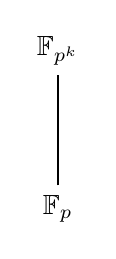
\begin{tikzpicture}
      \node (Fp) at (0, 0) {$\mathbb{F}_p$};
      \node (Fpk) at (0, 2) {$\mathbb{F}_{p^k}$};
      \draw (Fp) edge[edgetower] (Fpk);
    \end{tikzpicture}

    &   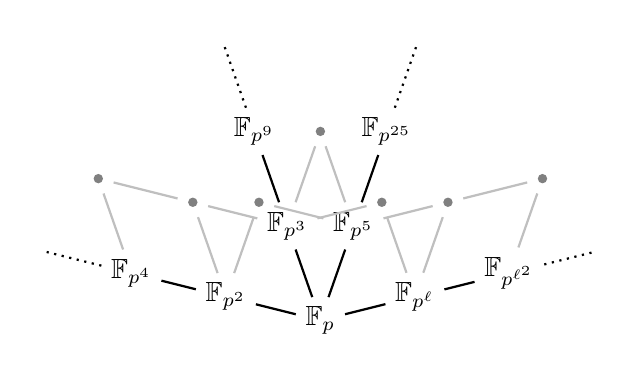
\begin{tikzpicture} [scale = 0.6] %, every node/.style={inner sep = 2pt, scale=0.8}]
    \coordinate (T2) at (-2, 0.5);
    \node (Fp) at (0, 0) {$\mathbb{F}_p$};
    \node (Fp2) at ($(Fp) + (T2)$) {$\mathbb{F}_{p^2}$};
    \node (Fp4) at ($(Fp2) + (T2)$) {$\mathbb{F}_{p^4}$};
    \node (Fp2l) at ($(Fp4) + (T2)$) {};% {$\FF_p^{(2)}$};
    % ---------------------
    \coordinate (T3) at (-0.7, 2);
    \uncover<1>{\node (Fp3) at ($(Fp) + (T3)$) {$\mathbb{F}_{p^3}$};}
    %\uncover<2>{\node[red] (Fp3) at ($(Fp) + (T3)$) {$\mathbb{F}_{p^3}$};}
    \node (Fp9) at ($(Fp3) + (T3)$) {$\mathbb{F}_{p^9}$};
    \node (Fp3l) at ($(Fp9) + (T3)$) {};% {$\FF_p^{(3)}$};
    % ---------------------
    \coordinate (T5) at (0.7, 2);
    \uncover<1>{\node (Fp5) at ($(Fp) + (T5)$) {$\mathbb{F}_{p^5}$};}
    %\uncover<2>{\node[red] (Fp5) at ($(Fp) + (T5)$) {$\mathbb{F}_{p^5}$};}
    \node (Fp25) at ($(Fp5) + (T5)$) {$\mathbb{F}_{p^{25}}$};
    \node (Fp5l) at ($(Fp25) + (T5)$) {};% {$\FF_p^{(5)}$};
    % ---------------------
    \coordinate (Tl) at (2, .5);
    \node (Fpl) at ($(Fp) + (Tl)$) {$\mathbb{F}_{p^\ell}$};
    \node (Fpl2) at ($(Fpl) + (Tl)$) {$\mathbb{F}_{p^{\ell^2}}$};
    \node (Fpll) at ($(Fpl2) + (Tl)$) {};% {$\FF_p^{(\ell)}$};
    % ---------------------
    \node[dotstyle] (dot1) at ($(Fp2) + (Fp3) - (Fp)$) {};
    \node[dotstyle] (dot2) at ($(Fp4) + (dot1) - (Fp2)$) {};
    \node[dotstyle] (dot3) at ($(Fp2) + (Fp5) - (Fp)$) {};
    \uncover<1>{\node[dotstyle] (dot4) at ($(Fp3) + (Fp5) - (Fp)$) {};}
    %\uncover<2>{\node[dotstyle, red] (dot4) at ($(Fp3) + (Fp5) - (Fp)$) {};}
    \node[dotstyle] (dot5) at ($(Fp3) + (Fpl) - (Fp)$) {};
    \node[dotstyle] (dot6) at ($(Fp5) + (Fpl) - (Fp)$) {};
    \node[dotstyle] (dot7) at ($(Fpl2) + (dot6) - (Fpl)$) {};
    % ---------------------
    \draw
    (Fp)
    edge[edgetower] (Fp2)
    edge[edgetower] (Fp3)
    edge[edgetower] (Fp5)
    edge[edgetower] (Fpl)
    (Fp2)
    edge[edgetower] (Fp4)
    edge[edgecomp] (dot1)
    (Fp4)
    edge[edgetower, dotted] (Fp2l)
    edge[edgecomp] (dot2)
    (dot1)
    edge[edgecomp] (dot2)
    (Fp3)
    edge[edgetower] (Fp9)
    edge[edgecomp] (dot1)
    edge[edgecomp] (dot4)
    (Fp9)
    edge[edgetower, dotted] (Fp3l)
    (Fp5)
    edge[edgetower] (Fp25)
    edge[edgecomp] (dot4)
    edge[edgecomp] (dot6)
    (Fp25)
    edge[edgetower, dotted] (Fp5l)
    (Fpl)
    edge[edgetower] (Fpl2)
    edge[edgecomp] (dot6)
    (Fpl2)
    edge[edgetower, dotted] (Fpll)
    edge[edgecomp] (dot7)
    (dot3)
    edge[edgecomp] (Fp2)
    edge[edgecomp] (Fp5)
    (dot5)
    edge[edgecomp] (Fp3)
    edge[edgecomp] (Fpl)
    (dot6)
    edge[edgecomp] (dot7);
  \end{tikzpicture} \\
  $\leadsto$ efficient \fvb{operations} & $\leadsto$ efficient \fvb{morphisms}
  \\
  in one given field & between fields
  \end{tabular}
\end{table}
\end{frame}

\begin{frame}{Contributions}
  Published in the \emph{International Symposium on Symbolic and Algebraic
  Computation} (ISSAC):
  \begin{itemize}
    \item \emph{Lattices of compatibly embedded finite fields in Nemo/Flint},
      Luca De Feo, Hugues Randriambololona, and É. R., 2018
    \item \emph{Standard lattices of compatibly embedded finite fields}, Luca De
      Feo, Hugues Randriambololona and É. R., 2019
  \end{itemize}
  Published in the \emph{International Workshop on the Arithmetic of Finite
  Fields} (WAIFI):
  \begin{itemize}
    \item \emph{Trisymmetric multiplication formulae in finite fields}, Hugues
      Randriambololona and É. R., 2020
  \end{itemize}
\end{frame}

\section{Single extension}
\subsection{Motivation}
\begin{frame}{Finite field arithmetic}
  \fvb{Notation:} $\mathbb{F}_{p^k}$ denotes \emph{the} finite field with $p^k$
  elements
  \[
    \mathbb{F}_{p^k} \cong \mathbb{F}_p[X]/(P(X))
  \]
  \begin{itemize}
    \item $P\in\mathbb{F}_p[X]$ is an \fvb{irreducible} polynomial of degree $k$
  \end{itemize}
  Some possible \fvb{representations}:
  \begin{itemize}
    \item \fvb{Zech's logarithm}: elements are represented as generator
      powers
    \uncover<2->{
      \begin{itemize}
        \item fast, but only possible for small fields
      \end{itemize}
    }
    \item \fvb{normal} basis: $(\alpha, \alpha^\sigma, \dots,
      \alpha^{\sigma^{k-1}})$
    \uncover<3->{
      \begin{itemize}
        \item fast Frobenius evaluation but slow multiplication
      \end{itemize}
    }
    \item \fvb{monomial} basis: $(1, \bar X, \dots, \bar X^{k-1})$
    \uncover<4->{
      \begin{itemize}
        \item commonly used representation, easy to construct
        \item multiplication slower than addition
      \end{itemize}
        }
  \end{itemize}
\end{frame}

\begin{frame}{Motivation}
  \begin{itemize}
    \item Computations in an extension $\mathbb{F}_{p^k}$% over $\mathbb{F}_p$
      \begin{itemize}
        \item<2-> multiplications: \fvb{expensive} \bad
        \item<2-> additions, scalar multiplications: \fvb{cheap} \good
      \end{itemize}
    \item<3-> we want to study/reduce the cost of multiplication
    \item<4-> A lot of litterature on the subject
      \begin{itemize}
        \item<5-> \fvb{Karatsuba} (1962)
        \item<6-> Toom-Cook (1963), \fvb{evaluation-interpolation} techniques
%        \item \fbv{CRT-}based algorithms
        \item<7-> \fvb{Schönhage-Strassen} (1971)
        \item<8-> \dots
        \item<9-> \comp{k\log k} algorithm \bib{Harvey, Van Der Hoeven}{19}
      \end{itemize}
  \end{itemize}
\end{frame}

\begin{frame}{Models of complexity}
  $\mathcal A$ an $\mathbb{F}_p$-algebra
  \begin{itemize}
      \item \fvb{algebraic} complexity: we count all operations $+, \times$ in $\mathbb{F}_p$
      \item \fvb{bilinear} complexity: we count only the multiplications
        \begin{itemize}
          \item nice results with polynomials: \fvb{Karatsuba's algorithm}
          \item and with matrices: \fvb{Strassen's algorithm}
        \end{itemize}
  \end{itemize}

  When $\mathcal A=\mathbb{F}_{p^k}$:
  \begin{itemize}
    \item theoretical interest
    \item links with coding theory
    \item links with algebraic geometry
  \end{itemize}
\end{frame}

\begin{frame}{Bilinear complexity: intuition}
  \begin{itemize}
    \item $\mathbb{F}_{p^k}$ an extension of $\mathbb{F}_p$
    \item \fvb{bilinear complexity:} number of subproducts in $\mathbb{F}_p$
      needed to compute a product in $\mathbb{F}_{p^k}$
  \end{itemize}
  \fvb{Karatsuba:}
\[(a_0+ a_1 X)(b_0 + b_1 X) = \]
\[
  \only<1>{a_0b_0+(a_0b_1+a_1b_0)X+a_1b_1X^2}
  \only<2>{\textcolor{red}{\mathbf{a_0b_0}}+(\frb{a_0b_1}+\frb{a_1b_0})X+\frb{a_1b_1}X^2}
  \only<3>{c_0+(c_2-c_1-c_0)X+c_1X^2}
  \only<4->{\frb{c_0}+(\frb{c_2}-\frb{c_1}-\frb{c_0})X+\frb{c_1}X^2}
\]
\uncover<3->{with
\[
  \left\{
  \begin{array}{lll}
   c_0 & = & a_0 b_0 \\
   c_1 & = & a_1 b_1 \\
   c_2 & = & (a_0+a_1) (b_0+b_1)
  \end{array}
  \right.
\]
}
\begin{itemize}
  \item<5-> \bad~\fvb{Hard} to compute the bilinear complexity of a product:
    unkwown even for the $3\times3$ matrix product
\end{itemize}
\end{frame}

\begin{frame}{Complexity of Karatsuba's algorithm}
  \begin{center}
  \only<1>{\includegraphics[scale=0.3]{img/karatsuba0.pdf}}
  \only<2>{\includegraphics[scale=0.3]{img/karatsuba1.pdf}}
  \only<3>{\includegraphics[scale=0.3]{img/karatsuba2.pdf}}
  \only<4>{\includegraphics[scale=0.3]{img/karatsuba3.pdf}}
  \only<5>{\includegraphics[scale=0.3]{img/karatsuba4.pdf}}
  \only<6>{\includegraphics[scale=0.3]{img/karatsuba5.pdf}}
  \only<7>{\includegraphics[scale=0.3]{img/karatsuba6.pdf}}
  \only<8>{\includegraphics[scale=0.3]{img/karatsuba7.pdf}}
  \only<9>{\includegraphics[scale=0.3]{img/karatsuba8.pdf}}
  \end{center}
  \begin{itemize}
    \item<2->Degree $2$: \fvb{$3$ multiplications instead of $4$}
    \item<3->Higher degrees: reccursive strategy
    \item<4->Asymptotically: \comp{n^{1.58}} instead of \comp{n^2}
  \end{itemize}
\end{frame}

\subsection{Bilinear complexity}
\begin{frame}{Bilinear complexity: definition}
  \begin{defi}
    The \fvb{bilinear complexity} of the product in $\mathbb{F}_{p^k}$ is the minimal integer
    $r\in\mathbb{N}$ such that you can write, for all $x,
    y\in\mathbb{F}_{p^k}$
    \[
      \only<1>{xy = \sum_{j=1}^r \alert<3->{\varphi_j(x)\psi_j(y)}\cdot\alpha_j}
      \only<2->{xy = \sum_{j=1}^r
      \alert<3->{\frb{\varphi_j(x)}\frb{\psi_j(y)}}\cdot\alpha_j}
    \]
    with $\varphi_j, \psi_j$ linear forms and $\alpha_j$ elements of
    $\mathbb{F}_{p^k}$.
  \end{defi}
  \begin{itemize}
    \item<2-> $\varphi_j(x)$: linear combination of the coordinates $x_i$ of $x$
    \item<2-> $\psi_j(y)$: linear combination of the coordinates $y_i$ of $y$
  \end{itemize}
\end{frame}

\begin{frame}{Notations and questions}
  \begin{itemize}
    \item $\mu_p(k) = $ bilinear complexity of the product in $\mathbb{F}_{p^k}$
  \end{itemize}

  \fvb{Two independent questions:}
  \begin{itemize}
    \item What is the asymptotic behaviour of $\mu_p(k)$?
      \begin{itemize}
        \item<2-> $\mu_p(k)$ is \fvb{linear} in $k$
        \item<3-> \fvb{Evaluation-interpolation} techniques:
          \begin{itemize}
            \item<4-> \bib{Chudnovsky-Chudnovsky}{87}
            \item<4-> \bib{Shparlinski-Tsfasman-Vladut}{92}
            \item<4-> \bib{Ballet}{99}
            \item<4-> \bib{Randriambololona}{12}
            \item<4-> \dots
          \end{itemize}
      \end{itemize}
    \item Can we find values $\mu_p(k)$ for small $k$?
      \begin{itemize}
        \item<5-> Clever exhaustive search~\bib{BDEZ}{12}~\bib{Covanov}{18}
      \end{itemize}
  \end{itemize}
\end{frame}

\subsection{Symmetries}
\begin{frame}{Symmetric decompositions}
\begin{table}
 \centering
  \begin{tabular}{c|c}
    \fvb{Classic} decompositions & \fvb{Symmetric} decompositions \\
    $xy=\sum_{j=1}^r \varphi_j(x)\psi_j(y)\cdot\alpha_j$ & $yx=xy=\only<1>{\sum_{j=1}^r
    \alert<2->{\varphi_j}(x)\alert<2->{\varphi_j}(y)\cdot\alpha_j}\only<2->{\sum_{j=1}^r
    \frb{\varphi_j}(x)\frb{\varphi_j}(y)\cdot\alpha_j}$
  \end{tabular}
\end{table}
\uncover<3->{\fvb{Notation:} for $\mathbb{F}_{p^k}$, we note
$\mu_p^\text{sym}(k)$ the minimal length $r$ in a \fvb{symmetric} decomposition}
\begin{itemize}
  \item<4->\fvb{Asymptotics:} $\mu_p^{\text{sym}}(k)$ is \fvb{linear} in $k$
  \item<5->\fvb{Small values:} \fvb{smaller} search space $\leadsto$ \fvb{faster} algorithms
\end{itemize}
\end{frame}

\begin{frame}{Even more symmetry}
  \begin{itemize}
    \item every linear form $\varphi\in(\mathbb{F}_{p^k})^\vee$ can be written $x\mapsto\Tr(\alpha x)$ for some
      $\alpha\in\mathbb{F}_{p^k}$, with $\Tr$ the trace of
      $\mathbb{F}_{p^k}/\mathbb{F}_p$
    \item we can rewrite the formula\uncover<3->{, and even ask
      $\beta_j=\lambda_j\alpha_j$}
  \end{itemize}
  \only<1>{
  \begin{equation*}
    xy = \sum_{j=1}^r \varphi_j(x)\varphi_j(y)\cdot\beta_j
  \end{equation*}}
\only<2>{
  \begin{equation*}
    xy = \sum_{j=1}^r \Tr(\alpha_jx)\Tr(\alpha_jy)\cdot\beta_j
  \end{equation*}}
\only<3>{
  \begin{equation*}
    xy = \sum_{j=1}^r\lambda_j
    \Tr(\alpha_jx)\Tr(\alpha_jy)\cdot\alpha_j
  \end{equation*}}
\only<4->{
  \begin{equation*}
    xy = \sum_{j=1}^r\lambda_j
    \Tr(\frb{\alpha_j}x)\Tr(\frb{\alpha_j}y)\cdot\frb{\alpha_j}
  \end{equation*}}

  \uncover<3->{with $\lambda_j\in\mathbb{F}_p$ scalars}
  \begin{itemize}
    \item<4-> we call these formulae \fvb{trisymmetric} decompositions
    \item<5-> we note $\mu_p^\text{tri}(k)$ the minimal $r$ in such formulae
  \end{itemize}
\end{frame}

\begin{frame}{Example of trisymmetric decomposition}
  \begin{itemize}
    \item $\mathbb{F}_{3^2} \cong \mathbb{F}_3[z]/(z^2-z-1)\cong
      \mathbb{F}_3(\zeta)$
    \item $x, y \in \mathbb{F}_{3^2}$, $x = x_0+x_1\zeta$ and $y=y_0+y_1\zeta$
      \uncover<2->{
      \[
        (x_0+x_1\zeta)(y_0+y_1\zeta) =
        (x_0y_0+x_1y_1)+(x_0y_1+x_1y_0+x_1y_1)\zeta
      \]
    }
  \end{itemize}
  \uncover<3->{
  \[
  \begin{array}{lll}
    xy &=& - \Tr(\textcolor<4->{blue}{1}\times
    x)\Tr(\textcolor<4->{blue}{1}\times y)\cdot\textcolor<4->{blue}{1}-
    \Tr(\textcolor<4->{red}{\zeta}\times
    x)\Tr(\textcolor<4->{red}{\zeta}\times y)\cdot\textcolor<4->{red}{\zeta}\\
    & & + \Tr((\textcolor<4->{orange}{\zeta-1})\times
    x)\Tr((\textcolor<4->{orange}{\zeta-1})\times y)\cdot(\textcolor<4->{orange}{\zeta-1})
  \end{array}
  \]
}
\uncover<4->{
  with
\[
  \left\{
  \begin{array}{lll}
    \Tr(x)\Tr(y) & = & (x_0-x_1)(y_0-y_1)\\
    \Tr((\zeta-1)x)\Tr((\zeta-1)y) & = & (x_0+x_1)(y_0+y_1) \\
    \Tr(\zeta x)\Tr(\zeta y) & = & x_0y_0
  \end{array}
  \right.
\]
}
\end{frame}

\begin{frame}{About trisymmetric decompositions}
  \fvb{Link with other decompositions:}
  \[
    \mu_p(k)\only<1>{\leq}\only<2->{\underset{?}{<}}\mu_p^\text{sym}(k)\only<1>{\leq}\only<2->{\underset{?}{<}}\mu_p^\text{tri}(k)
  \]
  \uncover<3->{
    \begin{prop}[Randriambololona, '14]
     Tri-symmetric decompositions always exist, except for $p=2, m\geq3$.
    \end{prop}
  }
  \uncover<4->{
  Results from \bib{Randriambololona, R.}{20}:
}
  \begin{itemize}
    \item<4-> \fvb{Asymptotics:} linearity in $k$ can be obtained for
      \fvb{symmetric multilinear} decompositions in $\mathbb{F}_{p^k}$
      \begin{itemize}
        \item<5-> Corollary: $\mu_p^\text{tri}(k)$ is also \fvb{linear} in $k$
      \end{itemize}
    \item<6-> \fvb{Small values:} usual algorithms do not work
      \begin{itemize}
        \item<7-> We provide an \textit{ad hoc} exhaustive search algorithm
      \end{itemize}
  \end{itemize}
\end{frame}

\begin{frame}{Partial conclusion}
  \fvb{Results:}
  \begin{itemize}
    \item Linearity of the \fvb{symmetric multilinear} complexity
    \item Linearity of the \fvb{trisymmetric} complexity
    \item New algorithm to find trisymmetric decompositions
  \end{itemize}
  \uncover<2->{
  \fvb{Future work:}
  \begin{itemize}
    \item Find better bounds for the linearity of $\mu_p^{\text{tri}}$
    \item Find algorithms exploiting the symmetries in the trisymmetric
      decompositions
  \end{itemize}
}
\end{frame}

\section{Many extensions}
\subsection{Context}
\begin{frame}{Context}
  \begin{itemize}
    \item Use of Computer Algebra System (CAS) 
    \item Use of many extensions of a prime finite field $\mathbb{F}_p$
    \item Computations in $\bar{\mathbb{F}}_p$.
  \end{itemize}
     \begin{figure}
  \centering
  \tikzset{
        dotstyle/.style={circle, inner sep = 1.2pt, outer sep = 4pt, fill =
        gray},
        edgetower/.style={thick},
        edgecomp/.style={thick, lightgray}
          }
  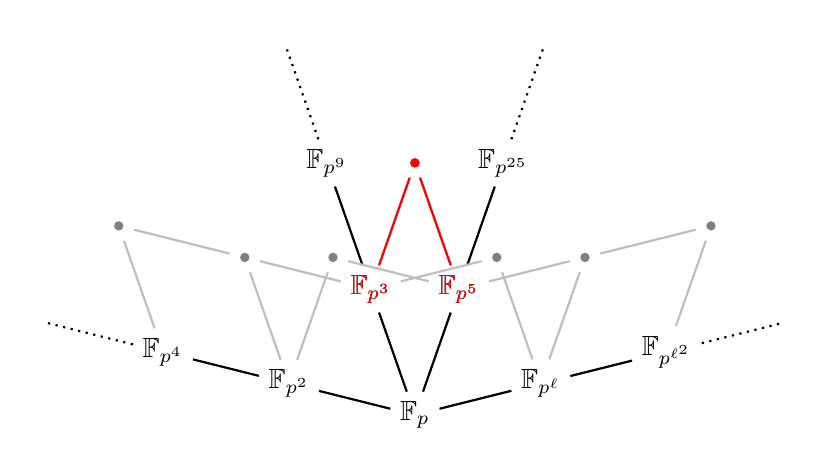
\begin{tikzpicture} [scale = 0.8] %, every node/.style={inner sep = 2pt, scale=0.8}]
    \coordinate (T2) at (-2, 0.5);
    \node (Fp) at (0, 0) {$\mathbb{F}_p$};
    \node (Fp2) at ($(Fp) + (T2)$) {$\mathbb{F}_{p^2}$};
    \node (Fp4) at ($(Fp2) + (T2)$) {$\mathbb{F}_{p^4}$};
    \node (Fp2l) at ($(Fp4) + (T2)$) {};% {$\FF_p^{(2)}$};
    % ---------------------
    \coordinate (T3) at (-0.7, 2);
    \uncover<1>{\node (Fp3) at ($(Fp) + (T3)$) {$\mathbb{F}_{p^3}$};}
    \uncover<2>{\node[red] (Fp3) at ($(Fp) + (T3)$) {$\mathbb{F}_{p^3}$};}
    \node (Fp9) at ($(Fp3) + (T3)$) {$\mathbb{F}_{p^9}$};
    \node (Fp3l) at ($(Fp9) + (T3)$) {};% {$\FF_p^{(3)}$};
    % ---------------------
    \coordinate (T5) at (0.7, 2);
    \uncover<1>{\node (Fp5) at ($(Fp) + (T5)$) {$\mathbb{F}_{p^5}$};}
    \uncover<2>{\node[red] (Fp5) at ($(Fp) + (T5)$) {$\mathbb{F}_{p^5}$};}
    \node (Fp25) at ($(Fp5) + (T5)$) {$\mathbb{F}_{p^{25}}$};
    \node (Fp5l) at ($(Fp25) + (T5)$) {};% {$\FF_p^{(5)}$};
    % ---------------------
    \coordinate (Tl) at (2, .5);
    \node (Fpl) at ($(Fp) + (Tl)$) {$\mathbb{F}_{p^\ell}$};
    \node (Fpl2) at ($(Fpl) + (Tl)$) {$\mathbb{F}_{p^{\ell^2}}$};
    \node (Fpll) at ($(Fpl2) + (Tl)$) {};% {$\FF_p^{(\ell)}$};
    % ---------------------
    \node[dotstyle] (dot1) at ($(Fp2) + (Fp3) - (Fp)$) {};
    \node[dotstyle] (dot2) at ($(Fp4) + (dot1) - (Fp2)$) {};
    \node[dotstyle] (dot3) at ($(Fp2) + (Fp5) - (Fp)$) {};
    \uncover<1>{\node[dotstyle] (dot4) at ($(Fp3) + (Fp5) - (Fp)$) {};}
    \uncover<2>{\node[dotstyle, red] (dot4) at ($(Fp3) + (Fp5) - (Fp)$) {};}
    \node[dotstyle] (dot5) at ($(Fp3) + (Fpl) - (Fp)$) {};
    \node[dotstyle] (dot6) at ($(Fp5) + (Fpl) - (Fp)$) {};
    \node[dotstyle] (dot7) at ($(Fpl2) + (dot6) - (Fpl)$) {};
    % ---------------------
    \draw
    (Fp)
    edge[edgetower] (Fp2)
    edge[edgetower] (Fp3)
    edge[edgetower] (Fp5)
    edge[edgetower] (Fpl)
    (Fp2)
    edge[edgetower] (Fp4)
    edge[edgecomp] (dot1)
    (Fp4)
    edge[edgetower, dotted] (Fp2l)
    edge[edgecomp] (dot2)
    (dot1)
    edge[edgecomp] (dot2)
    (Fp3)
    edge[edgetower] (Fp9)
    edge[edgecomp] (dot1)
    %edge[edgecomp] (dot4)
    (Fp9)
    edge[edgetower, dotted] (Fp3l)
    (Fp5)
    edge[edgetower] (Fp25)
    %edge[edgecomp] (dot4)
    edge[edgecomp] (dot6)
    (Fp25)
    edge[edgetower, dotted] (Fp5l)
    (Fpl)
    edge[edgetower] (Fpl2)
    edge[edgecomp] (dot6)
    (Fpl2)
    edge[edgetower, dotted] (Fpll)
    edge[edgecomp] (dot7)
    (dot3)
    edge[edgecomp] (Fp2)
    edge[edgecomp] (Fp5)
    (dot5)
    edge[edgecomp] (Fp3)
    edge[edgecomp] (Fpl)
    (dot6)
    edge[edgecomp] (dot7);
    \uncover<1>{\draw (Fp3) edge[edgecomp] (dot4);}
    \uncover<2>{\draw (Fp3) edge[thick, red] (dot4);}
    \uncover<1>{\draw (Fp5) edge[edgecomp] (dot4);}
    \uncover<2>{\draw (Fp5) edge[thick, red] (dot4);}
  \end{tikzpicture}
\end{figure}
\end{frame}

\begin{frame}{Embeddings}
  \begin{itemize}
    \item When $k\mid l$, we know $\mathbb{F}_{p^k}\emb\mathbb{F}_{p^l}$
      \begin{itemize}
        \item How to compute an embedding \fvb{efficiently}?
        \item There are several embeddings, \fvb{how to choose}?
      \end{itemize}
    \item Naive algorithm: if $\mathbb{F}_{p^k}=\mathbb{F}_p[x]/(P(x))$, find a
      root $\rho$ of $P$ in $\mathbb{F}_{p^l}$ and map $\bar x$ to $\rho$.
      Complexity strictly larger than \softcomp{k^2}.
    \item Lots of other solutions in the litterature:
      \begin{itemize}
        \item \bib{Lenstra}{91}
        \item \bib{Allombert}{02}
        \item \bib{Rains}{96}
        \item \bib{Narayanan}{18}
      \end{itemize}
  \end{itemize}
\end{frame}

\begin{frame}[fragile]{Compatibility}
  \begin{itemize}
    \item $\mathbb{F}_{p^{k}}, \mathbb{F}_{p^{l}}, \mathbb{F}_{p^{m}}$ three
      finite fields with $k\mid l\mid m$
    \item $f:\mathbb{F}_{p^{k}}\emb \mathbb{F}_{p^{l}}$,
      $g:\mathbb{F}_{p^{l}}\emb \mathbb{F}_{p^{m}}$,
      $h:\mathbb{F}_{p^{k}}\emb \mathbb{F}_{p^{m}}$ embeddings
\end{itemize}
\fvb{Compatibility:}

\begin{minipage}{0.2\textwidth}
  \vspace{12mm}
\begin{figure}
  \centering
    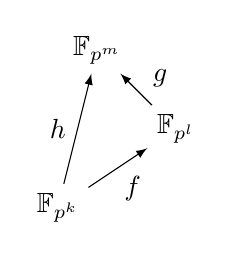
\begin{tikzpicture}
      \node (E) at (0, 0) {$\mathbb{F}_{p^{k}}$};
      \node (F) at (1.5, 1) {$\mathbb{F}_{p^{l}}$};
      \node (G) at (0.5, 2) {$\mathbb{F}_{p^{m}}$};

      \draw[arrow] (E) -- (F);
      \draw[arrow] (E) -- (G);
      \draw[arrow] (F) -- (G);

      \node (f12) at (0.95, 0.25) {$f$};
      \node (f13) at (0, 1) {$h$};
      \node (f23) at (1.3, 1.65) {$g$};
    \end{tikzpicture}
\end{figure}
\uncover<2->{
  \vspace{6mm}
  \[
    \textcolor{purple}{g\circ f \overset{?}{=} h}
  \]
}
\end{minipage}
\hspace{1mm}
\begin{minipage}{0.7\textwidth}
\begin{Verbatim}[commandchars=\\\{\}, fontsize=\scriptsize]
\textcolor{red}{In:}  p = 17; Fp = GF(p); FpX.<x> = Fp[]
     \textcolor{gray}{# We create finite fields of degree 12, 24, 48}
     P12, P24 = x^12 + x + 2, x^24 + x^2 + 2*x + 7
     P48 = x^48 + x^2 + 2*x + 6
     GFp12 = FiniteField(p^12, 'x12', modulus=P12)
     GFp24 = FiniteField(p^24, 'x24', modulus=P24)
     GFp48 = FiniteField(p^48, 'x48', modulus=P48)
     \textcolor{gray}{# We (naively) compute the roots we need}
     a = P12.any_root(GFp24) \textcolor{gray}{# Image of 'x12' in GFp24}
     b = P24.any_root(GFp48) \textcolor{gray}{# Image of 'x24' in GFp48}
     c = P12.any_root(GFp48) \textcolor{gray}{# Image of 'x12' in GFp48}
     a \textcolor{gray}{# We print 'a'} 
\textcolor{blue}{Out:} 6*x24^23 + 15*x24^22 + ... + 12*x24 + 16
  \end{Verbatim}
\pause{}
\begin{Verbatim}[commandchars=\\\{\}, fontsize=\scriptsize]
     \textcolor{gray}{# We map 'x24' to 'b'}
\textcolor{red}{In:}  c == a.polynomial()(b)
  \end{Verbatim}
\pause{}
\begin{Verbatim}[commandchars=\\\{\}, fontsize=\scriptsize]
\textcolor{blue}{Out:} False
\end{Verbatim}
\end{minipage}
\end{frame}

\begin{frame}{Ensuring compatibility: Conway polynomials}
  \begin{defi}[$l$-th Conway polynomials $C_l$]
    \begin{itemize}
      \item degree $l$, irreducible, monic
      \item primitive (\ie its roots generate $\mathbb{F}_{p^l}^\times$)
      \item \emph{norm-compatible} (\ie $C_k\left( X^{\frac{p^l-1}{p^k-1}}
        \right) = 0 \mod C_l$ if $k\,|\,l$)
    \end{itemize}
  \end{defi}
  \begin{itemize}
    \item<2-> \fvb{Standard polynomials}
    \item<3-> Compatible embeddings: $\bar{X}\mapsto
      \bar{Y}^{\frac{p^l-1}{p^k-1}}$\hspace{10mm}\softcomp{l^2}
    \item<4-> \textcolor{purple}{Hard to compute (exponential complexity)}
  \end{itemize}
\end{frame}
\subsection{Bosma, Canon and Steel's framework}
\begin{frame}{Ensuring compatibility: Bosma, Cannon and Steel}
  \begin{itemize}
    \item Framework originally used in MAGMA
    \item Based on the \fvb{naive embedding algorithm}
    \item Allows user-defined finite fields
    \item Computations made on the fly
  \end{itemize}
\end{frame}

\begin{frame}{Common subfield}
  \begin{itemize}
    \item Generalization of the naive algorithm
  \end{itemize}
     \begin{figure}
    \centering
    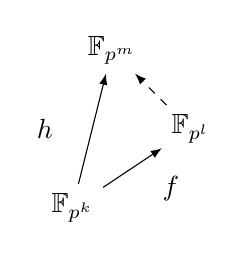
\begin{tikzpicture}
      \node (E) at (0, 0) {$\mathbb{F}_{p^{k}}$};
      \node (F) at (1.5, 1) {$\mathbb{F}_{p^{l}}$};
      \node (G) at (0.5, 2) {$\mathbb{F}_{p^{m}}$};

      \draw[arrow] (E) -- (F);
      \draw[arrow] (E) -- (G);
      \draw[dashed-arrow] (F) -- (G);

      \node (f12) at (1.25, 0.25) {$f$};
      \node (f13) at (-0.35, 1) {$h$};
    \end{tikzpicture}
  \end{figure}
  \begin{itemize}
    \item Consider $\alpha$ such that $\mathbb{F}_{p^{l}}=\mathbb{F}_p(\alpha)$
    \item Take $\rho$ a root of $h(\minpoly_{\mathbb{F}_{p^{k}}}(\alpha))$
    \item Map $\alpha\mapsto\rho$
%      \[
%        g(\sum_{i=0}^{l/k-1}e_i\alpha^i) =
%        \sum_{i=0}^{l/k-1}h(f^{-1}(e_i))\rho^i
%      \]
  \end{itemize}
  \begin{center}
    \fvb{We obtain $h = g\circ f$}
  \end{center}
\end{frame}

\begin{frame}{Several subfields}
  \begin{figure}
    \centering
    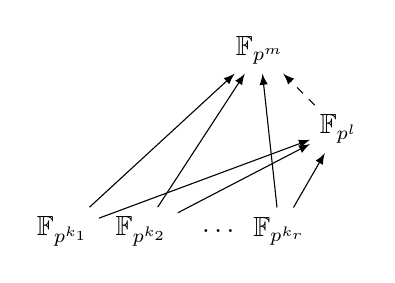
\begin{tikzpicture}
      \node (E1) at (-2, -.3) {$\mathbb{F}_{p^{k_1}}$}; 
      \node (E2) at (-1, -.3) {$\mathbb{F}_{p^{k_2}}$}; 
      \node (Er) at (0.75, -.3) {$\mathbb{F}_{p^{k_r}}$}; 
      \node (p) at (0, -.3) {$\dots$};
      \node (F) at (1.5, 1) {$\mathbb{F}_{p^{l}}$}; 
      \node (G) at (0.5, 2) {$\mathbb{F}_{p^{m}}$}; 

      \draw[arrow] (E1) -- (F);
      \draw[arrow] (E1) -- (G);
      \draw[arrow] (E2) -- (F);
      \draw[arrow] (E2) -- (G);
      \draw[arrow] (Er) -- (F);
      \draw[arrow] (Er) -- (G);
      \draw[dashed-arrow] (F) -- (G);
    \end{tikzpicture}
  \end{figure} 
  \begin{itemize}
    \item Consider $\alpha$ such that $\mathbb{F}_{p^{l}}=\mathbb{F}_p(\alpha)$
    \item Take $\rho$ a root of
      $\gcd_i(h_i(\minpoly_{\mathbb{F}_{p^{k_i}}}(\alpha)))$
    \item Map $\alpha\mapsto\rho$
    \item \fvb{This gives an embedding compatible with all subfields}
  \end{itemize}
\end{frame}

\begin{frame}{Implicit isomorphisms}
    From implicit isomorphisms come compatibility conditions
 \begin{center}
       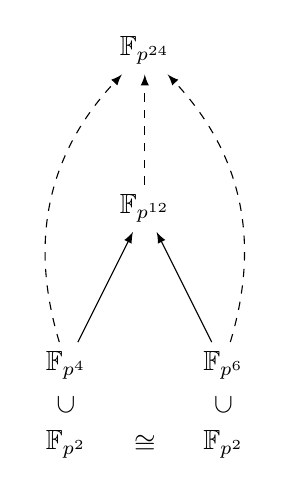
\begin{tikzpicture}
         \node (4) at (0, 0) {$\mathbb{F}_{p^{4}}$};
         \node (6) at (2, 0) {$\mathbb{F}_{p^{6}}$};
         \node (12) at (1, 2) {$\mathbb{F}_{p^{12}}$};
         \node (24) at (1, 4) {$\mathbb{F}_{p^{24}}$};
   
       \draw[arrow] (4) -- (12);
       \draw[arrow] (6) -- (12);
   
       \node[rotate=90] (sub1) at (0, -0.5) {$\subset$};
       \node[rotate=90] (sub2) at (2, -0.5) {$\subset$};
         \node (2) at (0, -1) {$\mathbb{F}_{p^{2}}$};
         \node (2bis) at (2, -1) {$\mathbb{F}_{p^{2}}$};
         \node (iso) at (1, -1) {$\cong$};
       \draw[dashed-arrow] (12) -- (24);
       \draw[dashed-arrow] (4) to[bend left] (24);
       \draw[dashed-arrow] (6) to[bend right] (24);
     \end{tikzpicture}
     \hspace{20mm}
     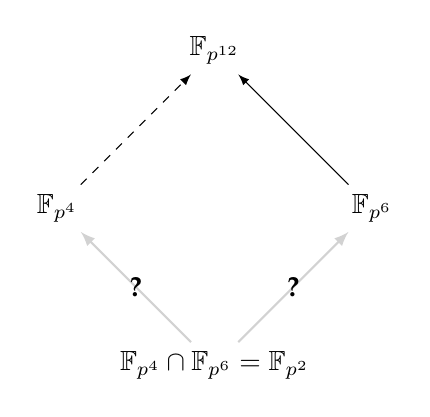
\begin{tikzpicture}
     \uncover<2->{
       \node (K) at (0, 2) {$\mathbb{F}_{p^{4}}$};
         \node (L) at (2, 4) {$\mathbb{F}_{p^{12}}$};
         \node (M) at (4, 2) {$\mathbb{F}_{p^{6}}$};

         \draw[dashed-arrow] (K) to (L);
         \draw[arrow] (M) to (L);
   }

         \uncover<3>{
         \node (I) at (2, 0) {$\mathbb{F}_{p^{4}}\cap
         \mathbb{F}_{p^{6}}=\mathbb{F}_{p^{2}}$};
         \draw[possible-arrow] (I) to (K);
         \draw[possible-arrow] (I) to (M);
         \node (1) at (1, 1) {\textbf{?}};
         \node (2) at (3, 1) {\textbf{?}};
       }
     \end{tikzpicture}
 \end{center}
\end{frame}

\begin{frame}{Computing the intersections}
  An example of what can happen with the intersections:
  \begin{figure}
    \centering
    \begin{tikzpicture}[scale=.8]

      \node (60) at (0, 0) {$\mathbb{F}_{p^{60}}$};
      \node (120) at (2, 2) {$\mathbb{F}_{p^{120}}$};
      \node (60) at (0, 0) {$\mathbb{F}_{p^{60}}$};
      \node (30) at (-2, -2) {$\mathbb{F}_{p^{30}}$};
      \node (40) at (4, 0) {$\mathbb{F}_{p^{40}}$};
      \node (6) at (-4, -4) {$\mathbb{F}_{p^{6}}$};

      \draw[arrow] (6) -- (30);
      \draw[arrow] (30) -- (60);
      \draw[arrow] (40) -- (120);
      \draw[dashed-arrow] (60) -- (120);

      \uncover<2->{
        \node (20) at (2, -2) {$\mathbb{F}_{p^{20}}$};
        \draw[arrow] (20) -- (40);
        \draw[dashed-arrow] (20) -- (60);
      }

      \uncover<3->{
        \node (10) at (0, -4) {$\mathbb{F}_{p^{10}}$};
        \draw[arrow] (10) -- (20);
        \draw[dashed-arrow] (10) -- (30);
      }

      \uncover<4->{
        \node (2) at (-2, -6) {$\mathbb{F}_{p^{2}}$};
        \draw[arrow] (2) -- (10);
        \draw[arrow] (2) -- (6);
      }

      \uncover<5->{
        \draw[arrow] (10) -- (30);
      }
      \uncover<6->{
        \draw[arrow] (20) -- (60);
      }
      \uncover<7->{
        \draw[arrow] (60) -- (120);
      }
    \end{tikzpicture}
  \end{figure}
\end{frame}

\begin{frame}{Results}
  \begin{itemize}
    \item Following~\bib{De Feo, Randriambololona, R.}{18},  Bosma-Canon-Steel
      framework is now part of the free Computer Algebra System \fvb{Nemo}
    \item It is practical but
      \begin{itemize}
        \item based on the naive embedding algorithm
          $\leadsto$~\fvb{superquadratic} complexity
        \item adding an extension is quadratic in the size of the lattice
      \end{itemize}
  \end{itemize}
  \fvb{Goals:}
  \begin{itemize}
    \item Change the embedding algorithm
    \item Lessen the cost of adding an extension
  \end{itemize}
\end{frame}

\subsection{Standard lattices}
\begin{frame}{Ideas}
  \begin{itemize}
    \item Plugging Allombert's embedding algorithm in Bosma, Cannon, and Steel
    \item Generalizing Bosma, Cannon, and Steel
    \item Generalizing Conway polynomials
  \end{itemize}
  \begin{center}
    \fvb{Bring the best of both worlds!}
  \end{center}
\end{frame}

\begin{frame}{Allombert's embedding algorithm}
  \begin{itemize}
    \item Based on \fvb{Kummer theory}
    \item For $k\,|\,(p-1)$, we work in $\mathbb{F}_{p^k}$, and
      study
  \end{itemize}
      \begin{equation}
        \tag{H90}
        \sigma(x) = \zeta_k x
        \label{h90}
      \end{equation}
      where $(\zeta_k)^k = 1$ and
      $\zeta_k\in\mathbb{F}_{p}\subset\mathbb{F}_{p^k}$
      \begin{itemize}
        \item When $k\mid l$ and $(\zeta_l)^{l/k}=\zeta_k$, from $\alpha_k\in\mathbb{F}_{p^{k}},
          \alpha_l\in\mathbb{F}_{p^{l}}$ solutions of~\eqref{h90}, we
          can deduce an \fvb{embedding} of the form
          \[
            \alpha_k\mapsto\kappa_{k, l}(\alpha_l)^{l/k}
          \]
          with $\kappa_{k, l}\in\mathbb{F}_p$ a constant
      \end{itemize}
\end{frame}

\begin{frame}{Allombert and Bosma, Canon, and Steel}
  \begin{itemize}
    \item Need to store one constant $\kappa_{k, l}$ for each pair
      $(\mathbb{F}_{p^k}, \mathbb{F}_{p^l})$
    \item The constant $\kappa_{k, l}$ depends on $\alpha_k$ and $\alpha_l$
  \end{itemize}
  \fvb{We would like to:}
  \begin{itemize}
    \item get rid of the constants $\kappa_{k, l}$ (\eg have $\kappa_{k, l}=1$)
    \item equivalently, get "standard" solutions of~\eqref{h90}
      \begin{itemize}
        \item select solutions $\alpha_k$, $\alpha_l$ that always define the
          same embedding
        \item such that the constants $\kappa_{k, l}$ are well understood
      \end{itemize}
  \end{itemize}
\end{frame}

\begin{frame}{Standard solutions}
  Let $k\mid l\mid p-1$, $(\zeta_l)^{l/k}=\zeta_k$
  \begin{itemize}
    \item $\alpha_k\in\mathbb{F}_{p^k}$ and $\alpha_l\in\mathbb{F}_{p^l}$
      solutions of \eqref{h90} for $\zeta_k$ and $\zeta_l$
    \item $(\forall k\mid l\mid p-1,\, \kappa_{k, l} = 1)$ implies $(\alpha_k)^k =
      (\alpha_l)^l=\zeta_{p-1}$
    \item We can use this property to define ``standard solutions''
  \end{itemize}
  \uncover<2->{
  \begin{defi}[Standard solution]
    Let $k\mid p-1$ and $\alpha_k\in \mathbb{F}_{p^k}$ a solution
   of~\eqref{h90} for $\zeta_k=(\zeta_{p-1})^{\frac{p-1}{k}}$, $\alpha_k$ is
   \fvb{standard} if $(\alpha_k)^k = \zeta_{p-1}$.
  \end{defi}
}
\uncover<3->{
  \begin{defi}[Standard polynomial]
   All standard solutions $\alpha_k$ define the same irreducible
   polynomial of degree $k$, we call it the \fvb{standard polynomial} of
   degree $k$.
  \end{defi}
}
\end{frame}

\begin{frame}{Standard embeddings}
  Let $k\mid l\mid p-1$, $(\zeta_l)^{l/k}=\zeta_k$
  \begin{itemize}
    \item $\alpha_k$ and $\alpha_l$ \fvb{standard solutions} of~\eqref{h90} for
      $\zeta_k$ and $\zeta_l$
      \begin{itemize}
        \item<2-> $\kappa_{k, l} = 1$
      \end{itemize}
    \item<3-> The embedding
      \[
      \alpha_k\mapsto(\alpha_l)^{l/k}
    \]
    is \fvb{standard} too (only depends on $\zeta_{p-1}$).
  \end{itemize}
\end{frame}

\begin{frame}{What happens when $k\nmid p-1$?}
  Let $p\nmid k$ and $k\nmid p-1$
  \begin{itemize}
    \item no $k$-th root of unity $\zeta_k$ in $\mathbb{F}_{p}$
      \begin{itemize}
        \item \fvb{add them!} Consider
          $A_k=\mathbb{F}_{p^k}\otimes\mathbb{F}_{p}(\zeta_k)$ instead of
          $\mathbb{F}_{p^k}$
      \end{itemize}
\end{itemize}
      \begin{equation}
        \tag{H90'}
        (\sigma\otimes1)(x) = (1\otimes\zeta_k)x
        \label{h90'}
      \end{equation}
      \begin{itemize}
        \item Allombert's algorithm still works!
          \end{itemize}
          If $k\mid l$ and $(\zeta_l)^{l/k}=\zeta_k$
          \begin{itemize}
        \item Still possible to find \fvb{standard solutions} $\alpha_k,
          \alpha_l$ of \eqref{h90'}
        \item $\kappa_{k, l}\neq1$ but easy to compute
        \item \fvb{Standard embedding} from
              $\alpha_k$ and $\alpha_l$
      \end{itemize}
\end{frame}

\begin{frame}{Scheme of our work}
 \begin{figure}
  \centering
    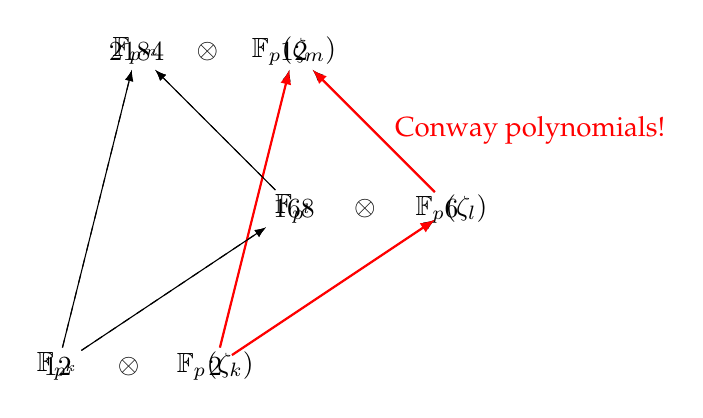
\begin{tikzpicture}
      \uncover<1-5>{
      \node (l) at (0, 0) {$\mathbb{F}_{p^k}$};
      \node (m) at (3, 2) {$\mathbb{F}_{p^l}$};
      \node (n) at (1, 4) {$\mathbb{F}_{p^m}$};
    }
      \uncover<6->{
      \node (l) at (0, 0) {$12$};
      \node (m) at (3, 2) {$168$};
      \node (n) at (1, 4) {$2184$};
    }

      \uncover<2->{
      \node (a) at (.9, 0) {$\otimes$};
      \node (b) at (3.9, 2) {$\otimes$};
      \node (c) at (1.9, 4) {$\otimes$};
    }

      \uncover<2-5>{
      \node (a) at (2, 0) {$\mathbb{F}_p(\zeta_k)$};
      \node (b) at (5, 2) {$\mathbb{F}_{p}(\zeta_l)$};
      \node (c) at (3, 4) {$\mathbb{F}_{p}(\zeta_m)$};
    }

      \uncover<6->{
      \node (a) at (2, 0) {$2$};
      \node (b) at (5, 2) {$6$};
      \node (c) at (3, 4) {$12$};
    }

   \uncover<-4>{
      \draw[dashed-arrow] (l) -- (m);
      \draw[dashed-arrow] (l) -- (n);
      \draw[dashed-arrow] (m) -- (n);
    }

      \uncover<3>{
      \draw[arrow] (a) -- (b);
      \draw[arrow] (a) -- (c);
      \draw[arrow] (b) -- (c);
    }

      \uncover<4->{
      \draw[arrow, red, thick] (a) -- (b);
      \draw[arrow, red, thick] (a) -- (c);
      \draw[arrow, red, thick] (b) -- (c);
      \node[red] (conway) at (6, 3) {Conway polynomials!};
    }

    \uncover<5->{
      \draw[arrow] (l) -- (m);
      \draw[arrow] (l) -- (n);
      \draw[arrow] (m) -- (n);
    }

    \end{tikzpicture}
\end{figure}
\uncover<6->{
  \begin{center}
  Example of degrees involved in the case $p=5$.
  \end{center}
}
 
\end{frame}

\begin{frame}{Compatibility and complexity}
  Results from~\bib{De Feo, Randriambololona, R.}{19}:
  \begin{prop}[Compatibility]
    Let $k\mid l\mid m$ and $f:\mathbb{F}_{p^k}\emb\mathbb{F}_{p^l}$,
    $g:\mathbb{F}_{p^l}\emb\mathbb{F}_{p^m}$, 
    $h:\mathbb{F}_{p^k}\emb\mathbb{F}_{p^m}$ the standard embeddings. Then we
    have $g\circ f = h$.
  \end{prop}
  \begin{prop}[Complexity]
    Given a collection of Conway polynomials of degree up to $d$, for any
  $k\mid l\mid p^i-1$, $i\leq d$
    \begin{itemize}
      \item Computing a standard solution $\alpha_k$ takes \softcomp{k^2}
      \item Given $\alpha_k$ and $\alpha_l$, computing the standard embedding
        $f:\mathbb{F}_{p^k}\emb \mathbb{F}_{p^l}$ takes \softcomp{l^2}
    \end{itemize}
  \end{prop}
\end{frame}

\begin{frame}{Implementation}
  Implementation using Flint/C and Nemo/Julia.
 \begin{figure}[h]
  \centering
  \includegraphics[scale=1]{img/plot_solve_h90.eps}
  \includegraphics[scale=1]{img/plot_embed.eps}
  \caption{Timings for computing $\alpha_k$ (left, logscale), and for computing
    $\mathbb{F}_{p^2}\emb\mathbb{F}_{p^k}$
    (right, logscale) for $p=3$.}
\end{figure}
\end{frame}

\begin{frame}{Conclusion, open problems}
  \begin{itemize}
    \item We implicitly assume that we have \fvb{compatible roots} $\zeta$ (\ie
      $\zeta_k = (\zeta_{l})^{l/k}$ for $k\mid l$)
      \begin{itemize}
        \item In practice, this is done using \fvb{Conway polynomials}
      \end{itemize}
    \item With Conway polynomials up to degree $d$, we can compute embeddings to
      finite fields up to any degree $k\mid p^i-1$, $i\leq d$
      \begin{itemize}
        \item quasi-quadratic complexity
      \end{itemize}
  \end{itemize}
  \fvb{Open problems:}
  \begin{itemize}
    \item Make this work less standard, but more practical
    \item Can we replace the Conway polynomials by other polynomials?
  \end{itemize}
\end{frame}

\begin{frame}
  \begin{center}
    \fvb{\Huge{Thank you!}}
  \end{center}
\end{frame}
\end{document}
